\documentclass[12pt,letterpaper]{article}
\usepackage{fullpage}
\usepackage[top=2cm, bottom=4.5cm, left=2.3cm, right=2.3cm]{geometry}
\usepackage{amsmath,amsthm,amsfonts,amssymb,amscd}
\usepackage{lastpage}
\usepackage{enumerate}
\usepackage{fancyhdr}
\usepackage{mathrsfs}
\usepackage{xcolor}
\usepackage{graphicx}
\usepackage{listings}
\usepackage{hyperref}

\hypersetup{%
  colorlinks=true,
  linkcolor=blue,
  linkbordercolor={0 0 1}
}
\usepackage{wrapfig}
\renewcommand\lstlistingname{Algorithm}
\renewcommand\lstlistlistingname{Algorithms}
\def\lstlistingautorefname{Alg.}

\lstdefinestyle{Python}{
    language        = Python,
    frame           = lines, 
    basicstyle      = \footnotesize
}

\setlength{\parindent}{0.0in}
\setlength{\parskip}{0.05in}

% Edit these as appropriate
\newcommand\course{CS 639}

%\pagestyle{fancyplain}
\headheight 35pt
\usepackage{xcolor}
% hyperref link defaults to "blue" (0000ff) as this matches our publisher produced pdf style
\definecolor{xlinkcolor}{cmyk}{1,1,0,0}
\usepackage{hyperref}
\fancypagestyle{firstpage}{
  \chead{\textbf{\Large  Bayesian vs Frequentist Approach \\in Medical Research \\}}
  \rhead{\course \\ \today}
  \lhead{ Harsh Sahu\\Lekshmi Thulasidharan }
  \lfoot{}
  \cfoot{}
  \rfoot{\small\thepage}
  \headsep 3em
}


\usepackage{amsmath}
\PassOptionsToPackage{hyphens}{url}
\fancypagestyle{normal}{
  %\renewcommand{\headrulewidth}{0.5pt}
  \headsep 3em
}

% Set the default page style to 'normal'
%\pagestyle{headings}
%\headsep 2em
%\fancyhead[R]{\rightmark}
%\renewcommand{\subsectionmark}[1]{\markright{#1}}

\pagestyle{headings}
\headsep 2em

%% In response to request from AAS 

\begin{document}
\par
%\thispagestyle{fancy}
\thispagestyle{firstpage}
\section{Introduction}
In medical research, statistical methods are commonly used to analyze data and draw conclusions. Two common approaches are the Bayesian and frequentist approaches. In simple words, Bayesian statistics involves the use of past/existing knowledge (a.k.a prior) along with the new data to make predictions, while frequentist statistics involves making inferences based on the observed data alone. We start this review with a comprehensive overview of each approach followed by a comparison study. Specifically, we try to answer the following questions:
\begin{itemize}
    \item What are the relative strengths and weaknesses of Bayesian and frequentist methods in the context of medical research?
    \item  Under which circumstances do the two approaches lead to similar or different conclusions?
    \item Does the use of one of these approaches increase the potential for breakthroughs in medical research compared to the other?
    \item What are the drawbacks of each approach?
\end{itemize}
We then review the application of Bayesian and frequentist methods in predicting the risk of dementia in older adults. 
\subsection{Frequentist Approach}

The frequentist approach considers probability of an event as the frequency of an event occuring in a large sample of data or repeated sampling of the same experiment. The basic idea is to evaluate the parameters of interest of the data which is not known. If we have a large sample of data, then we can choose the most likely value of the parameter which generates a similar data. This method is also called the Maximum Likelihood parameter estimation (MLE). 

\subsection{Bayesian Approach}
explain the foundations
\subsection{Comparison}
Also talk about medical research application. Case study : Dementia

\section{Application of frequentist approach in risk prediction of dementia in older adults}
Dementia is a common yet severe condition that primarily affects elder population. This is an umbrella term for conditions which could impair a person's ability to perform day to day activities since it has a detrimental effect on their cognition. For example, those who have dementia will experience memory loss, difficulty with communication and reasoning along with changes in psychological health. Unfortunately, there is currently no known cure for dementia. For this reason, it is extremely important to identify the individuals who are at very high risk for dementia early on, since this allows for incorporating lifestyle changes and treatments which could potentially slow the rate of progression of this condition. A straightforward method which allows the early identification of risk factors of dementia is by utilising statistical techniques to generate a risk score model. Researchers assign a score to every possible risk factors including demographic factors that could contribute to the development of dementia. Once we have the model, we can screen people and classify them into low, moderate and high risk populations. Within the frequentist approach, one statistical technique that can be highly effective in creating risk prediction models is the ``Logistic regression''. Here we review Barnes et al. (2009), where they developed one such risk score model i.e., a late life dementia index which can be used to accurately predict the chances of a person developing dementia in 6 years based on several risk factors using Logistic Regression. The tool they developed can be used to classify individuals into low, moderate and high risk categories for dementia, and hence serves as an excellent aid for monitoring vulnerable adults for dementia symptoms to start their treatment early on.  

\subsection{Logistic Regression}

\begin{wrapfigure}{r}{7cm}
\vspace{-7 mm}
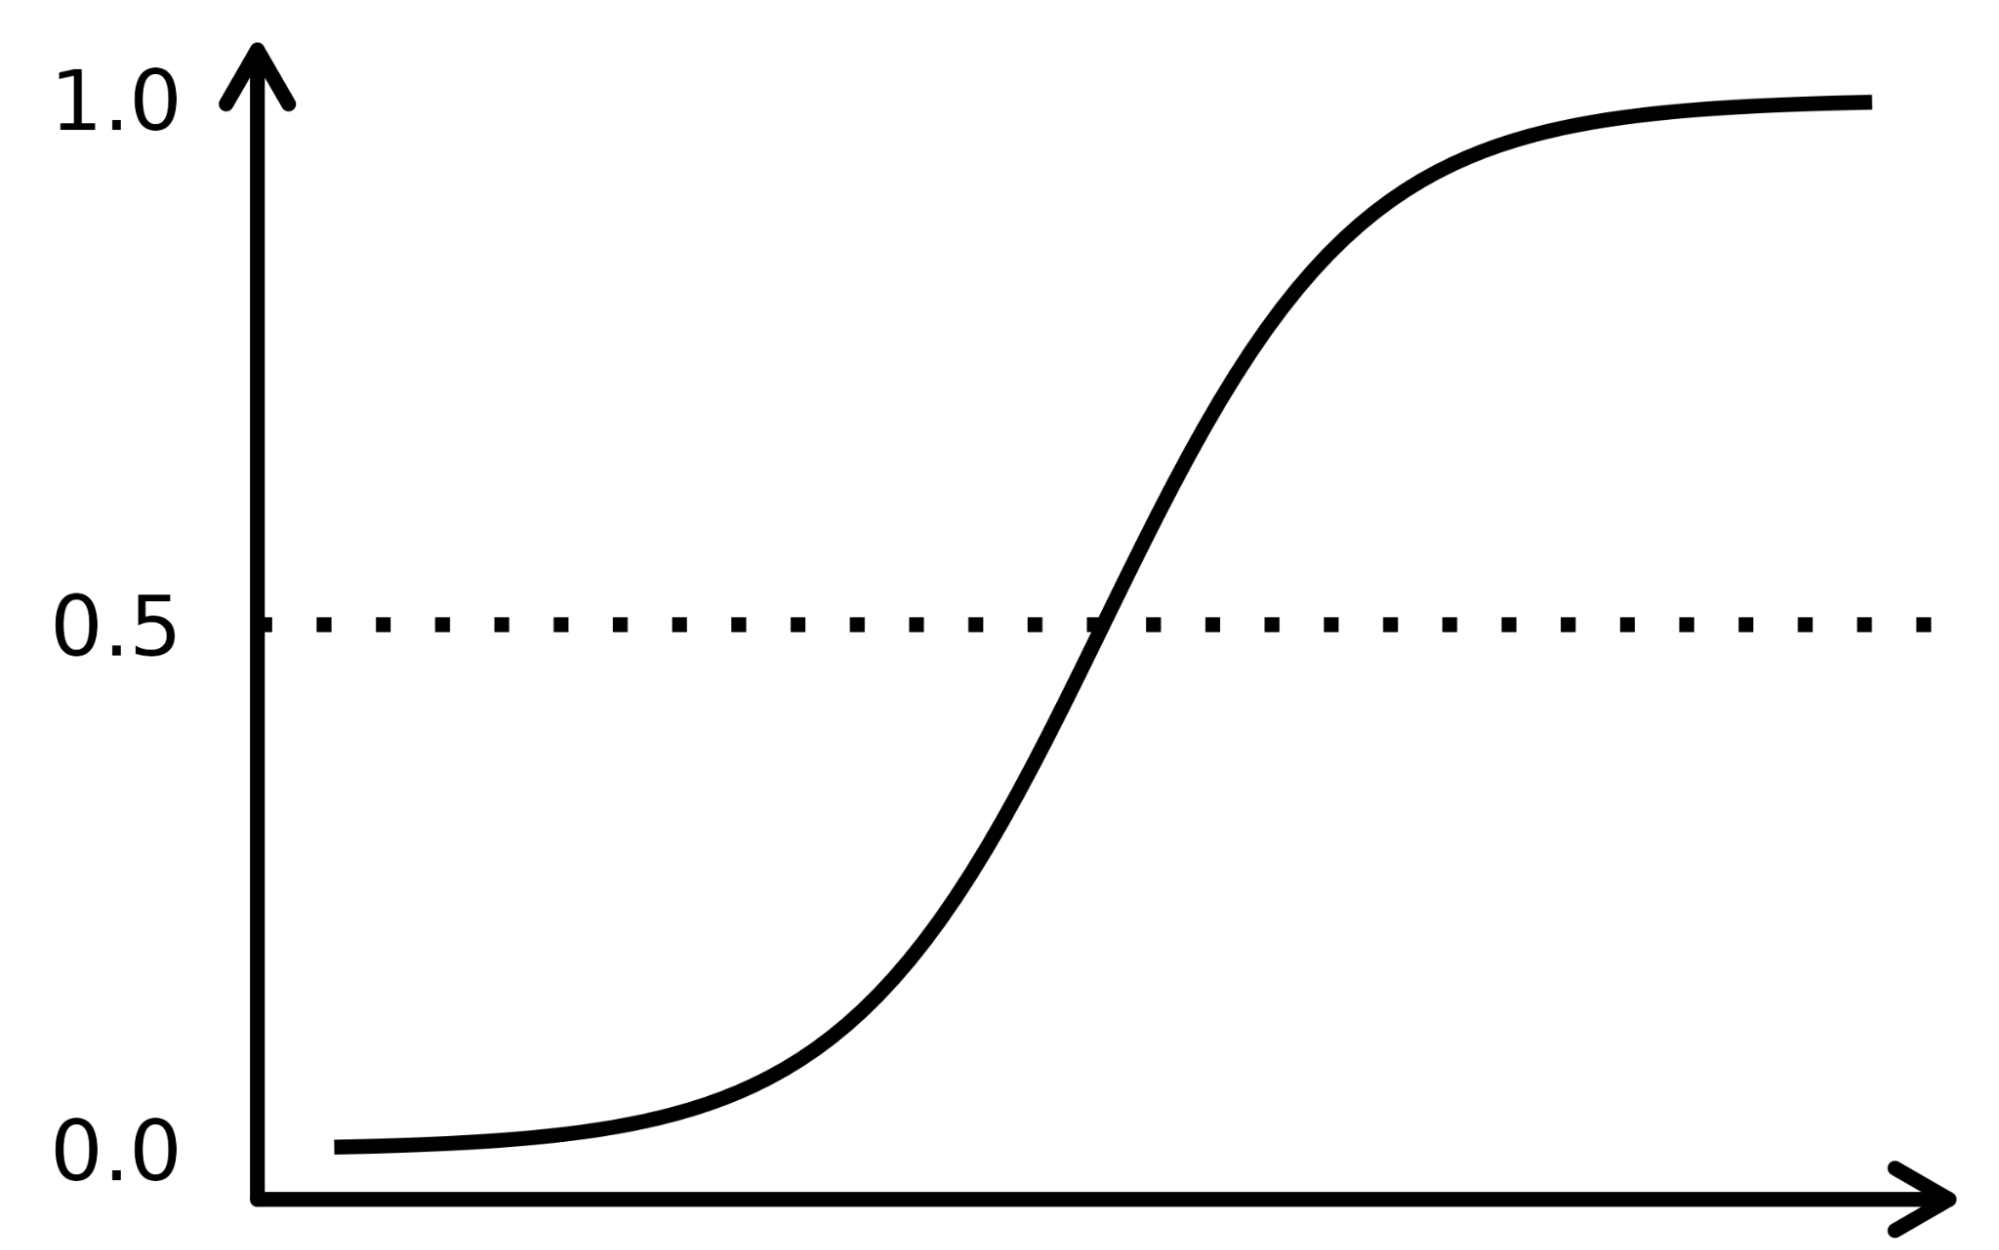
\includegraphics[width=7 cm]{sigmoid.png}
\caption{The sigmoid function curve}
\label{dvdr}
\end{wrapfigure}
Logistic Regression is a useful method for classification problems where we want to find the probability of a variable belongs to a particular category. So, this analysis is best for predicting binary outcomes like yes or no. In medical research this could translate into the probability of a patient developing a disease given one or more input variables (which would be the suspected risk factors). The probability is modelled using a logistic function which is a sigmoid (Fig.\ref{dvdr}) . The function takes a linear combination of the input variables and  and returns an output between 0 and 1. \\

When we have multiple input variables as in the case of risk prediction of a disease, the logistic function takes the form:
\begin{equation}
p(X) =Pr (Y|X)= \frac{e^{\beta_0+\beta_1X_1+\beta_2X_2+...+\beta_pX_p}}{1+e^{\beta_0+\beta_1X_1+\beta_2X_2+...+\beta_pX_p}}
\end{equation}

In the context of the paper we are discussing here, $Pr (Y|X)$ would the probability of a person developing dementia (modelled with variable $Y$) given certain risk factors (or predictors) assumed to be independent with each other($X=(X_1,X_2,\dots,X_p)$). The $\beta$ coefficients represent the parameters of the model, with $\beta_0$ being the intercept and $\beta_1,\beta_2,\dots,\beta_p$ being the coefficients for each of the independent variables. The coefficients can be estimated by maximizing the corresponding likelihood function.  

\subsection{Predictors of Dementia}

The data for different predictors were collected from the Cardiovascular Health Cognition Study which was started in 1989–1990 and updated during 1992–1993. They identified and classified individuals into three groups: (i) Those who already had dementia at the time of data collection, (ii) those who developed dementia after the data collection and (iii) those who developed mild cognitive impairment or MCI (this is not as severe as dementia) any time during the follow up period that lasted until 1998-1999. For this study, since the authors are interested in predicting the risk of dementia, they excluded individuals who belonged to the first category as well as those people who either died or lost contact before the follow up data is collected. This resulted in a sample size of 3,375. 

The authors consider a wide range of predictors for this study and they broadly belong to several categories described below:

(i) Demographic factors - This will help us understand if the risk of developing dementia is related to a person's age, gender, race, ethnicity, income etc.\\
(ii) Pre-exisitng medical conditions: Some of the medical conditions such as a history of stroke, diabetes etc. are known to increase the chances of a person developing dementia. \\
(iii)  Cognitive function : Cognitive function include a person's ability to learn, remember, reason, pay attention etc.  Since dementia is associated with a deterioration of cognitive abilities, this is a very important predictor of this condition. \\
(iv) Physical function measures: This is related to one's ability to perform normal day to day activities such as being able to get out of bed, eat, bath, walk, lift, carry weights etc without anyone's help. Since dementia is associated with weakened muscle strength and poor coordination, this is a very important risk factor.        \\            
(v) Physical performance measures: Some of the early symptoms of dementia involve taking more than usual time to perform certain normal activities. For eg. an individual could take more time to button or unbutton a shirt. So it is important to consider physical performance as a predictor.\\
(vi) Lifestyle factors: This involves information about one's alcohol consumption rate, smoking habits, time spent on exercise etc., which are indicators of how healthy a person is. \\
(vii) Psychosocial factors: This takes into consideration, a person's emotional and mental well-being. \\
(viii) Cerebral MRI variables: Includes the presence of small or large tumors, white matter disease (damage to white matter of the brain usually associated with aging) etc. that could seriously affect a person's coordination.\\
(ix) Carotid artery ultrasound variables and Electrocardiogram measurements: Considering this could possibly unveil any correlation of dementia with one's cardiovascular health.\\
(x) Genetic factors: Studies have shown that the presence of APOE polymorphic alleles in the genes makes a person at the risk of Alzheimer disease which comes under dementia.\\
(xi) Serum measures: Certain blood tests could help understand the underlying condition that causes change in a person's ability to think, reason and remember. \\

This is in fact a lot of predictors. But not all of them will contribute to dementia equally. Some of them could be very good indicators whereas some won't have any effect at all. So before using Logistic Regression to evaluate the finalized logistic coefficients to develop a late life dementia risk score, it makes sense to eliminate some of these predictors from the analysis based on their statistical significance. To do this, careful and rigorous statistical analysis techniques should be used. In the next section, we will look into the methodology followed by the authors to choose the subset of relevant predictors.

\subsection{Methodology for Statistical Analysis}

Before doing any high level statistics to determine the relationship between predictor variables and the target variable (i.e. dementia) using the data of the former, we should always start simple. That is, first step should be to understand the observed data itself. For the entire sample size, we should start by  looking at the distribution of data for every single predictors. This is as simple as plotting a histogram which tells us about the frequency distribution of the variable under study along with its mean, median, range etc. Doing this will help us identify any outliers in the data and also help us quantify what ``high'' and ``low'' means for every variable. In other words, we can identify the cut off value for every variable above which the value of variable is too high and below which it is too low. This will aid us in categorization of individuals for every predictors. For eg. based on the distribution of age of the sample population used in the paper, range is from 65-100 years. A cut off was applied at 74 and 79 to divide the population into three groups- 65-74, 75-79 and 80-100. This is essential because some symptoms which are predictive of dementia could be simply a part of natural process of aging. So dividing the population based on age will help in removing any such biases and improve the accuracy of the analysis.\\

It is very important to categorize the variables before looking at their association with dementia. Doing this will not only make it easy to identify existing patterns but also make the data more interpretable by being able to visualize it better. Categorization is a trivial thing to do when the variable we are considering is qualitative. For eg: Among the predictor variables that comes under demographic factors is the gender. It is essential to categorize individuals into biological male and female populations to study the association with dementia. It may not be so straightforward if the variable in the question is quantitative. For eg: one of the risk factors of dementia is poor physical performance when it comes to normal activities. A person who is under high risk of this disease might takes longer time to button a shirt compared to normal people.  Let's say the data of the time taken by a person to button a shirt consists of numbers ranging from 20 sec to 100 sec. To divide the data into what is normal and what is not, we need to determine the cut off point. Let's say normal time to button a shirt is $\leq45$ sec. In this case, we can simply divide the data into two categories by applying the cut off at $45$ sec. We don't need to consider every data point and this makes it easier to study the associations, if any, with dementia. So, it is crucial to accurately determine the cut off as any errors will have the potential to change the distribution of data of the respective groups and this will affect the accuracy of our risk prediction. When it comes to medical research, for some variables, the standard clinical cut off points are available. For eg: total cholesterol $<200$ mg/dL is normal and anything above this is considered high. For those variables which doesn't have such a cut off available, the authors apply the Classification and Regression Tree analysis or CART.\\
\begin{wrapfigure}{r}{7cm}
\vspace{-7 mm}
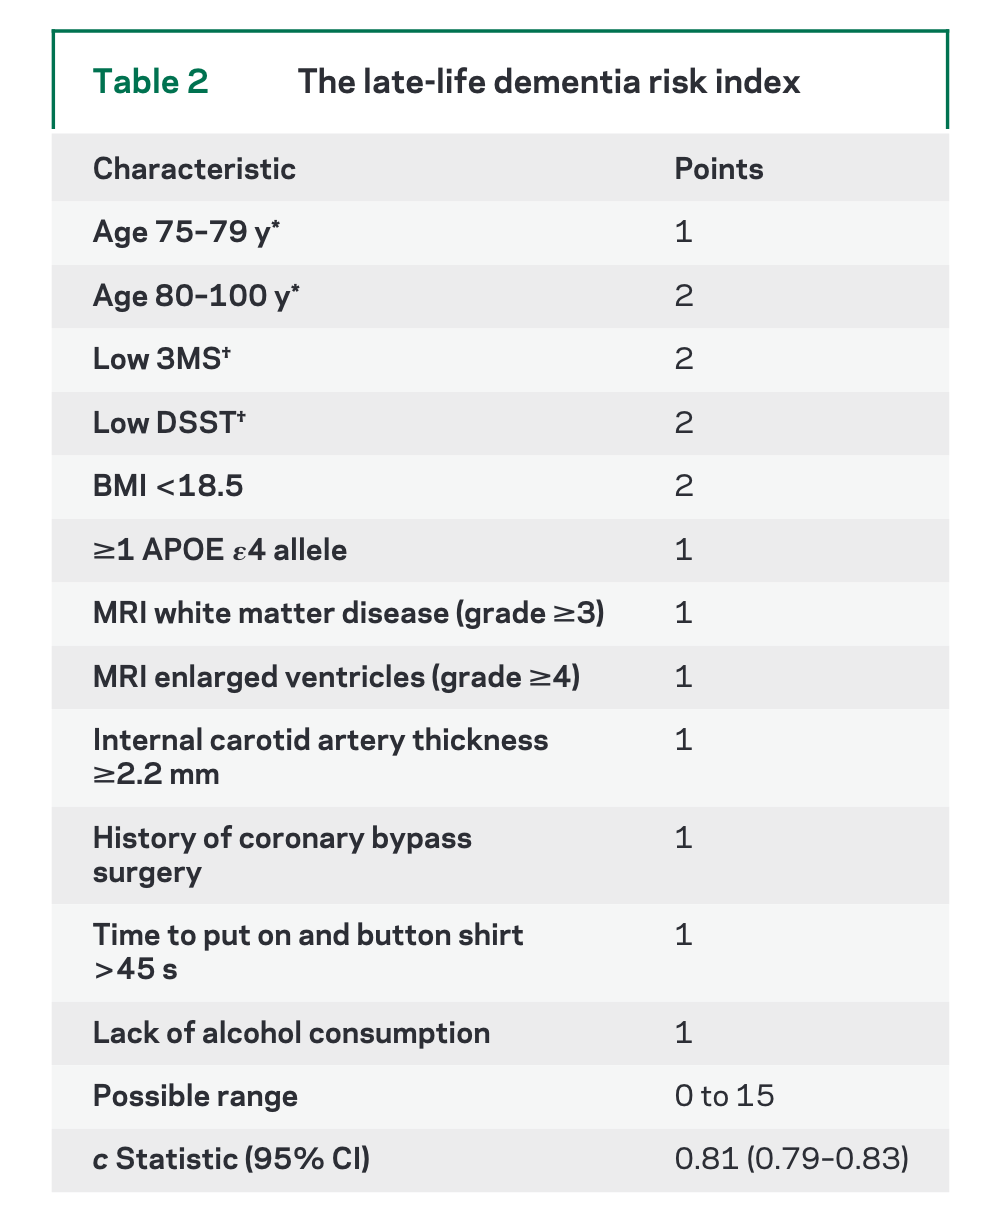
\includegraphics[width=7cm]{riskindex.png}
\caption{Late-life dementia risk index}
\label{risk}
\end{wrapfigure}
CART is a decision tree algorithm. In this study this is used to identify the cut points for the variables that best differentiate the output of interest, i.e., dementia or no dementia. They used it for both continuous variables such as blood pressure, age etc. and those which are categorical like alcohol consumption (none, moderate. high). The idea is to divide the data based on ``homegeneity". That is CART algorithm will recursively consider all possible cut points in the data for a given predictor variable and divide the data by choosing the optimum cut point that is associated with dementia/no dementia response. The optimum cut point is determined by calculating $\chi^2$ value for the groups of data generated and the output of interest, for every possible cut point. What does a $\chi^2$ test tells us? The idea is to compare the observed data to the expected data provided the null hypothesis is true. In this analysis, the null hypothesis would be ``The distribution of people who have dementia is the same in all categories of a particular variable". The distribution under null hypothesis would be our expected distribution. We are looking for the cut point which maximizes the $\chi^2$, i.e, the degree of difference between the different groups for a particular variable is maximum in this case. In the context of a  hypothesis test, this corresponds to rejecting the null hypothesis with a $p-$value less than the chosen significance $\alpha$. The authors used $\alpha=0.05$. \\

While doing the classification of predictors using CART, sometimes none of the cut points will be able to reject the null. Such predictor variables are removed before proceeding to the next step. Second step involves re-calculating the $p-$values after adjusting for demographics. Like I mentioned before while talking about classifying the population based on age, doing this is important because it helps in removing any biases associated with demographic factors. The number of predictors will further go down as correcting for demography will make some of them statistically insignificant. Once again, a bivariate analysis is done to determine the relationship between dementia risk and the predictors, but this time in categories (as in section 2.2). For every category, the variable which is most predictive of dementia is identified and then plugged into Eq.1, to calculate the logistic coefficients using multi-linear logistic regression. Here, we consider the effect of all the variables together. So it is possible to overfit the model if there are so many predictors. It is therefore important to make sure that only the most important predictors are included in our model. For this reason, the authors use a mixture of forward and backward sample selection procedure. The idea is simple. They started with no variables in the model, then add each predictors one by one and calculates the $p-$value of each variable in the model every time we add a new variable to make sure that all the variables maintain a $p-$ value below certain significance. If at any time, the $p-$ value of a variable rises above this threshold, that variable is removed from the model. Once the model is finalized, the logistic coefficients are calculated.\\

\subsection{Developing the risk index}
The logistic coefficients (denoted by $\beta$) are a measure of how strong the relationship is between the predictor variables and the outcome of interest. Larger the value of $\beta$, stronger is the relationship and vice versa. If the coefficient is positive, it means that the predictor and the outcome is positively correlated. If the coefficient is negative, that means their relationship is negatively correlated. In this work, the authors assigned those predictors with magnitude of coefficients $>0.75$, 2 points and those with magnitude of logistic coefficients $\leq0.75$ 1 point, to create a table of late-life risk index (see Fig.\ref{risk}).\\

\subsection{Accuracy of the model}

\begin{wrapfigure}{r!}{7cm}
\vspace{-11 mm}
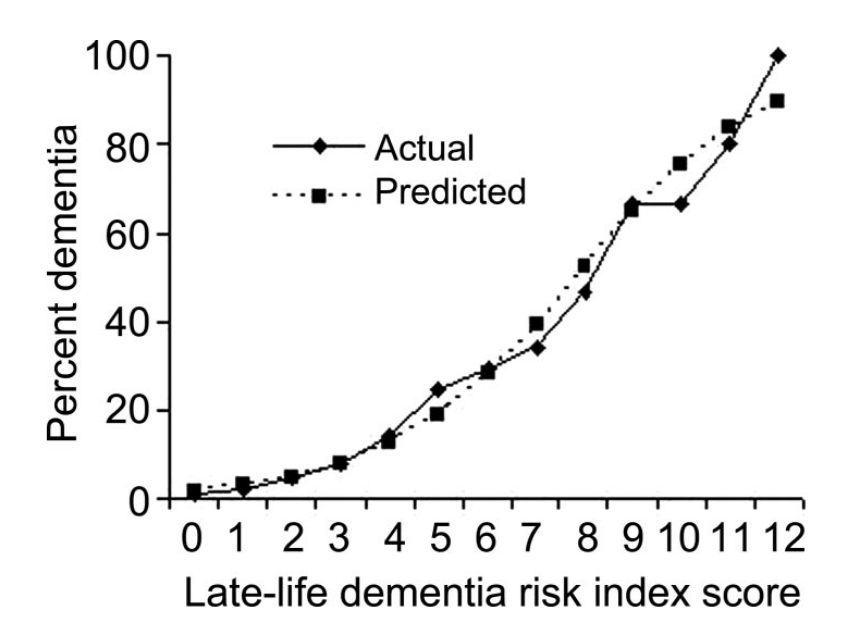
\includegraphics[width=7 cm]{riskplot.png}
\caption{Calibration of the late-life dementia risk index}
\label{plotrisk}
\end{wrapfigure}

The predictive accuracy of the model is quantified using $c-$ statisitc. $c-$ statistics shows the extent of goodness-of-fit of the model. They plot the true positive rate against false positive rate i.e, the risk score of a random person in the sample who has dementia vs risk score of random person who doesn't have dementia. Then the $c-$ statistic shows the probability of the former having a larger risk compared to the latter. From Fig.\ref{risk}, this probability is around 0.8. That implies a strong model.  In addition to this, the authors plotted the predicted percentage and the actual percentage of people who developed dementia against their risk index score calculated from Fig.\ref{risk}. It is very clear from Fig.\ref{plotrisk} that, the model is quite accurate in risk prediction of dementia.  In addition to this, it is very important to do validation. In  predictive models, validation helps in estimating how good the trained model is with the new data. Low error on training data set doesn't guarantee low error on test data as it possible to get low errors on the former if the model is overfitting the data. Among several techniques to validate the model, the authors use $k-$ fold Cross Validation. The training dataset itself is randomly divided into $k$ groups of equal size. Then the first fold is considered as a test data set and the rest $k-1$ of them the training set. This process is repeated over every folds to generate $k$ estimates of test error. An illustrative diagram is shown in Fig. \ref{cv} The paper uses 10 fold Cross validation and $c-$ statistic to quantify the test error.

\begin{figure}[t!]
\centering
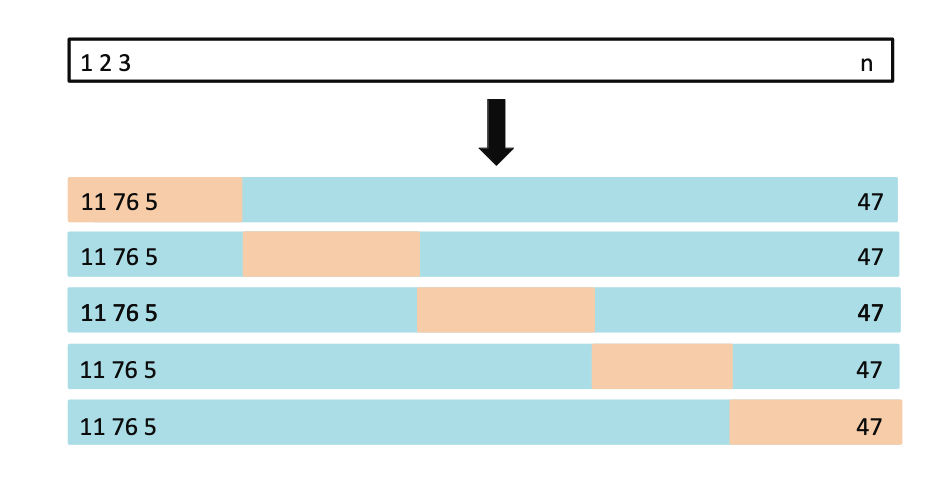
\includegraphics[width=15cm]{CV.png}
\caption{Diagram showing the process of $k-$ fold Cross Validation. Here the data is divided into 5 folds, so $k=5$. For the pupose of this study, the authors set $k=10$. }
\label{plotrisk}
\end{figure}
\subsection{Discussion}

This study is focused on developing a dementia risk index for people who belong to the age group $\geq 65$. Though the initial sampling population consists of people who belong to the age range 65-100, the study found that the number of people who developed dementia belonged to the age group of 65-74 is statistically insignificant. So the final risk index consists of people who are older than 74. Among a huge range of predictors, using rigorous statistical analysis based on Logistic Regression, the authors narrowed down the most important predictors of dementia after correcting for the demographic factors and assigned them points based on the magnitude of logistic coefficients. With the risk index, one can calculate the risk index by summing up the points assigned to the predictor variables. 0 points corresponds to no risk of dementia and 15 points corresponds to a high risk domain. It is shown that the predictive model they developed shows high accuracy in categorizing individuals based on dementia risk through the results observed after 6 years during the follow up period. The 12 most important predictors chosen by statistics under which the model is based on, are among the most predictive factors for dementia shown by clinical research. \\

World Health Organization, in their website says that more than 55 million people worldwide has dementia. It is estimated that more than 6 million Americans have Alzheimer's disease which is a type of dementia. With this being the case, the study uses data of patients who belongs to four US counties with a sample size of 3,375. This is a quite small sample compared to the population who actually has dementia. Also may be it was better to randomly sample individuals across the whole nation instead of just four regions. In addition to this, the study even though it considers African Americans, the accuracy of this model when applied to people who are from other countries should be investigated.  Other than this, in my opinion, this study is quite comprehensive and exhaustive. The authors were very meticulous in selecting the most important predictor variables which helped them avoid overfitting their model. They eliminated the predictors at different stages of their analysis based on the $p-$ values and made sure the $p-$ values of variables in their model at every stage of their study were always below the chosen significance. They also quantified the accuracy of their model using $c-$ statistics and validated their model using the standard Cross validation approach. It might be interesting to apply the bayesian statistics to the same data and see what the risk index table looks like.


\section{Bayesian Approach to identifying potential risk factors for Dementia}
This study aims to identify new potential risk factors for dementia using Bayesian statistics, based on nationwide longitudinal population-based data from Taiwan's National Health Insurance Research Database (NHIRD).

The study verifies 4 recognized risk factors for dementia:
\begin{itemize}
\item Severe head injury
\item Depression
\item Diabetes Mellitus
\item Vascular Diseases
\end{itemize}

Additionally, the study also found hearing loss and senile cataract as new potential risk factors for dementia.


The use of Bayesian statistics in medical research, including clinical trials, epidemiology, meta-analyses, and evidence synthesis, has become increasingly popular in recent years. Bayesian statistics is a way to combine past (prior) and present (current study) evidence to make decisions about the future (posterior conclusions). By using Bayesian statistics, this study was able to identify new potential risk factors for dementia and help clinicians develop appropriate treatment strategies for patients at the early stages of dementia and prevent the worsening of the condition.

\subsection{Data and Study Design}
\begin{figure}[t]
\centering
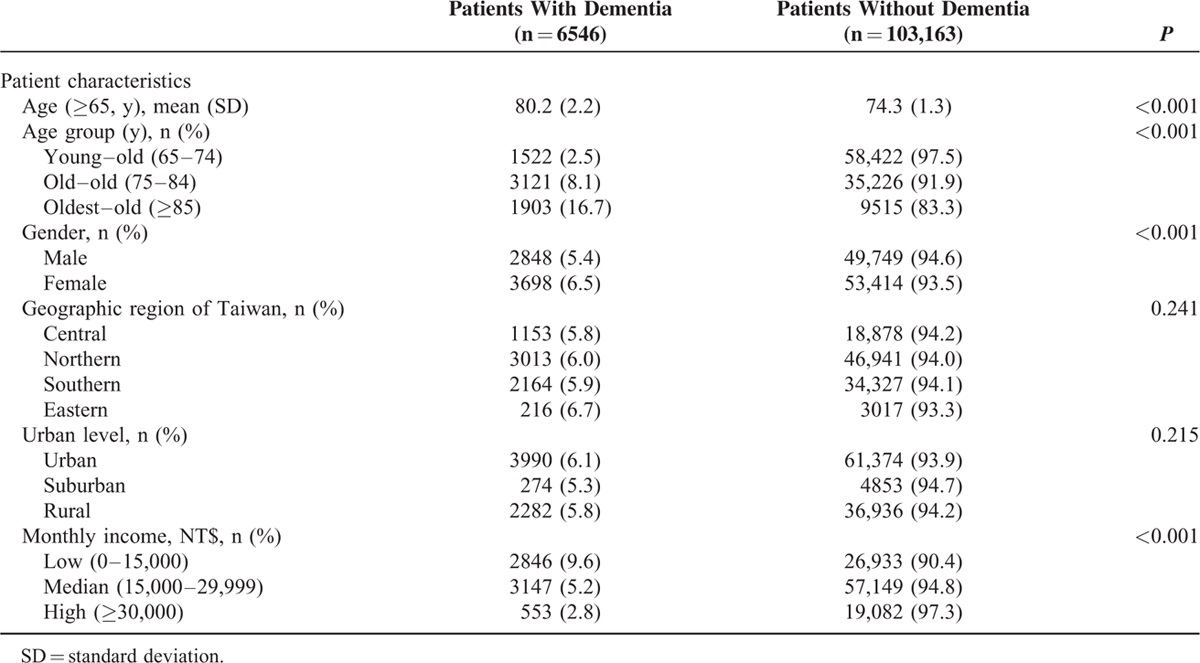
\includegraphics[width=1\linewidth]{bayesian_table1.jpeg}
\label{fig:bayesian_table1}
\caption{Demographics of the population}
\end{figure}

Of the 1,000,000 patients screened, we included 109,709 (11.0$\%$) patients aged $\geq 65$ years. A total of 6546 (6.0$\%$) patients were diagnosed with dementia. Figure 2 shows the distribution of sociodemographic characteristics of the study population. Patients with dementia were significantly older than those without dementia (80.2 years vs 74.3 years). Moreover, the percentage of patients with dementia in the young–old (65–74 years), old–old (75–84 years), and oldest–old ($\geq$85 years) groups was significantly increased by 2.5$\%$, 8.1$\%$, and 16.7$\%$, respectively. The percentage of women with dementia was significantly higher than that of men with dementia (n = 3698, 6.5$\%$ vs 2848, 5.4$\%$). Furthermore, patients with high income had a significantly lower incidence of dementia than in those with lower income (2.8$\%$, 5.2$\%$, and 9.6$\%$).

\subsection{Statistical Analysis}
The study derives the odds ratio (OR) by using the Bayesian approach. They attempt to learn about the unknown
distribution from given data, to make some inferences about certain properties of the distribution, and to determine the relative likelihood that each possible distribution is actually the correct one. Suppose that proportion $\theta$
of patients with dementia in a population in the presence of a risk factor is unknown, and let the prior distribution assigned to $\theta$ be a uniform distribution at the interval (0, 1); that is, the prior p.d.f. $\mathbb{P}(\theta) = 1$ for $0 < \theta < 1$. This “informationless” prior assignment is for the sake of objective purpose and reducing computing cost. Suppose there is a given random sample of n persons who all have a risk factor, and for $i = 1, 2, \dots, n$, let $X_i = 1$ if the $i_{th}$ person has dementia and let $X_i = 0$ otherwise. Then, $X_1, X_2, \dots, X_n$ form $n$ Bernoulli trials with parameter $\theta$. We can determine
the posterior p.d.f. of $\theta$.

\subsection{Results}
The study found that older age, female sex, and lower income were independent risk factors for dementia. The study also reidentified four recognized risk factors for dementia: vascular diseases, depression, severe head injury, and diabetes mellitus (DM). The study found that hearing loss and senile cataract were associated with an increased risk for dementia.

The study also highlighted that Taiwan has been an aging country since 1993, and the prevalence of dementia in the older population from 1995 to 2010 was approximately 6\%, similar to that in other developed countries. The study's results were consistent with previous studies, which identified older age, female sex, and lower socioeconomic status as risk factors for dementia in the East.

The study also highlighted the increasing evidence that increased risks of dementia are associated with treatable medical comorbidities, such as severe head injury, depression, DM, and vascular diseases. The study hypothesized that poor hearing and poor eyesight (senile cataract) are associated with an increased risk of dementia in older people. The study found that hearing loss and senile cataract are potential risk factors for dementia in the Taiwanese population.

In summary, the study identified several potential risk factors for dementia in the older population in Taiwan, using Bayesian statistics. The study's results were consistent with previous studies and highlighted the importance of addressing treatable medical comorbidities in reducing the risk of dementia.


\section{Evaluating Bayesian and Frequentist Approach on a Dataset}

\end{document}
